\documentclass[aspectratio=169,11pt,xcolor={dvipsnames,table}]{beamer}

% ============================================================================
% PACKAGES & THEME SETUP
% ============================================================================
\usepackage[utf8]{inputenc}
\usepackage[T1]{fontenc}
\usepackage{lmodern}
\usepackage{amsmath,amssymb,amsfonts,mathtools}
\usepackage{graphicx}
\usepackage{booktabs}
\usepackage{multirow}
\usepackage{makecell}
\usepackage{array}
\usepackage{ragged2e}
\usepackage{listings}
\usepackage{tikz}
\usepackage{pgfplots}
\pgfplotsset{compat=1.18}
\usetikzlibrary{shapes.geometric, arrows.meta, positioning, calc, fit, backgrounds, matrix}

% Theme & Color Palette (3-4 cohesive colors: Blue, Orange, Green, Dark Slate)
\usetheme{Madrid}
\usecolortheme{default}
\setbeamertemplate{navigation symbols}{}
\setbeamertemplate{blocks}[default]

\definecolor{PrimaryBlue}{HTML}{1E4E79}
\definecolor{AccentBlue}{HTML}{2B6CB0}
\definecolor{LightBlue}{HTML}{EBF4FF}
\definecolor{PrimaryOrange}{HTML}{C05621}
\definecolor{AccentOrange}{HTML}{DD6B20}
\definecolor{LightOrange}{HTML}{FFF5F0}
\definecolor{DarkSlate}{HTML}{1A202C}
\definecolor{MutedGray}{HTML}{4A5568}
\definecolor{SoftGray}{HTML}{F7FAFC}
\definecolor{BorderGray}{HTML}{CBD5E0}
\definecolor{SuccessGreen}{HTML}{2F855A}
\definecolor{LightGreen}{HTML}{F0FFF4}

% Dark IDE Code Colors (VS Code Dark+ / One Dark Palette)
\definecolor{CodeDarkBg}{HTML}{1E1E2E}
\definecolor{CodeFg}{HTML}{CDD6F4}
\definecolor{CodeKeyword}{HTML}{89B4FA}
\definecolor{CodeFunc}{HTML}{FAB387}
\definecolor{CodeType}{HTML}{F9E2AF}
\definecolor{CodeString}{HTML}{A6E3A1}
\definecolor{CodeComment}{HTML}{6C7086}

\setbeamercolor{palette primary}{bg=PrimaryBlue,fg=white}
\setbeamercolor{palette secondary}{bg=AccentBlue,fg=white}
\setbeamercolor{palette tertiary}{bg=DarkSlate,fg=white}
\setbeamercolor{structure}{fg=PrimaryBlue}
\setbeamercolor{frametitle}{bg=PrimaryBlue,fg=white}
\setbeamercolor{title}{bg=PrimaryBlue,fg=white}

% Vertically Middle-Aligned Table Column Types
\newcolumntype{L}[1]{>{\raggedright\arraybackslash}m{#1}}
\newcolumntype{C}[1]{>{\centering\arraybackslash}m{#1}}

% University Logo Watermark at Top-Right Corner of All Content Slides (Slides 2..19)
\addtobeamertemplate{frametitle}{}{%
  \vspace*{-0.38cm}%
  \begin{tikzpicture}[remember picture, overlay]
    \begin{scope}[shift={($(current page.north east)+(-0.62cm,-0.44cm)$)}]
      \fill[white, opacity=0.95] (0,0) circle (0.36cm);
      \clip (0,0) circle (0.35cm);
      \node[inner sep=0pt, opacity=0.92] at (0,0) {
\includegraphics[width=0.70cm,height=0.70cm]{../en/frontMatter/Logo_UET.png}};
    \end{scope}
  \end{tikzpicture}%
}

% Clean custom footline
\setbeamertemplate{footline}{
  \leavevmode%
  \hbox{%
  \begin{beamercolorbox}[wd=.28\paperwidth,ht=2.4ex,dp=1ex,left]{author in head/foot}%
    \hspace*{2ex}\usebeamerfont{author in head/foot}\textbf{Pham Nhat Minh} (VNU-UET)
  \end{beamercolorbox}%
  \begin{beamercolorbox}[wd=.54\paperwidth,ht=2.4ex,dp=1ex,center]{title in head/foot}%
    \usebeamerfont{title in head/foot}Weekly Report -- Document Key Information Extraction
  \end{beamercolorbox}%
  \begin{beamercolorbox}[wd=.18\paperwidth,ht=2.4ex,dp=1ex,right]{date in head/foot}%
    \usebeamerfont{date in head/foot}Slide \insertframenumber{} / \inserttotalframenumber\hspace*{2ex}
  \end{beamercolorbox}}%
  \vskip0pt%
}

% Strict Non-Hyphenation
\hyphenpenalty=10000
\exhyphenpenalty=10000

% Dark-Theme Python Syntax Highlighting Style (No Borders, No Line Seams)
\lstdefinestyle{pydark}{
    language=Python,
    basicstyle=\ttfamily\fontsize{6.2pt}{8.5pt}\selectfont\color{CodeFg},
    keywordstyle=\bfseries\color{CodeKeyword},
    commentstyle=\itshape\color{CodeComment},
    stringstyle=\color{CodeString},
    emph={self,torch,nn,F,mean,cat,clamp,unsqueeze,squeeze,zeros,sigmoid,forward,_segment_pool_and_contextualize,_compute_boundary_loss,binary_cross_entropy_with_logits,hierarchical_proj,segment_context,boundary_classifier,token_classifier,classifier,is_first_token_embedding},
    emphstyle=\bfseries\color{CodeFunc},
    emph={[2]Tensor,Optional,Tuple,int,float,Module,TokenClassifierOutput},
    emphstyle={[2]\bfseries\color{CodeType}},
    frame=none,
    linewidth=\linewidth,
    aboveskip=0pt,
    belowskip=0pt,
    xleftmargin=0pt,
    xrightmargin=0pt,
    showstringspaces=false,
    breaklines=true,
    columns=flexible
}

\begin{document}

% ============================================================================
% SLIDE 1: TITLE SLIDE (TOP-MIDDLE LOGO, CENTERED NAME CARDS)
% ============================================================================
\begin{frame}[plain]
  \vspace*{0.12cm}
  \begin{center}
    
\includegraphics[height=1.32cm]{../en/frontMatter/Logo_UET.png}\\[0.14cm]
    {\footnotesize\bfseries\color{MutedGray} UNIVERSITY OF ENGINEERING AND TECHNOLOGY\\[0.05cm] VIETNAM NATIONAL UNIVERSITY HANOI}\\[0.22cm]
    
    
\begin{tikzpicture}
      \node[draw=PrimaryBlue, fill=PrimaryBlue, rounded corners=7pt, inner sep=10pt, text width=12.6cm, minimum height=2.1cm, align=flush center] {
        {\Large\bfseries\color{white} Research on Enhancing Vision-Language Model\\[0.12cm] for Document Key Information Extraction}\\[0.16cm]
        {\normalsize\bfseries\color{LightBlue} Weekly report}
      };
    \end{tikzpicture}
    
    \vspace{0.26cm}
    
\begin{tikzpicture}
      \node[draw=BorderGray, fill=SoftGray, rounded corners=6pt, line width=0.9pt, inner sep=8pt, text width=5.85cm, minimum height=1.95cm, align=flush center] (pres) at (-3.32, 0) {
        {\footnotesize\bfseries\color{MutedGray} Presenter}\\[0.08cm]
        {\normalsize\bfseries\color{PrimaryBlue} Pham Nhat Minh}\\[0.08cm]
        {\scriptsize\color{DarkSlate} Major: Information Systems}
      };
      \node[draw=PrimaryOrange!70, fill=LightOrange, rounded corners=6pt, line width=0.9pt, inner sep=8pt, text width=5.85cm, minimum height=1.95cm, align=flush center] (sup) at (3.32, 0) {
        {\footnotesize\bfseries\color{PrimaryOrange!85} Supervisor}\\[0.08cm]
        {\normalsize\bfseries\color{PrimaryOrange} PhD. Pham Thi Quynh Trang}\\[0.08cm]
        {\scriptsize\color{DarkSlate} Faculty of Information Technology, \mbox{VNU-UET}}
      };
    \end{tikzpicture}
  \end{center}
\end{frame}

% ============================================================================
% SLIDE 2: TABLE OF CONTENTS (UNIVERSAL CARD SIZES, SYMMETRICALLY ALIGNED)
% ============================================================================
\begin{frame}{Table of Contents}
  \vspace{0.02cm}
  \begin{center}
    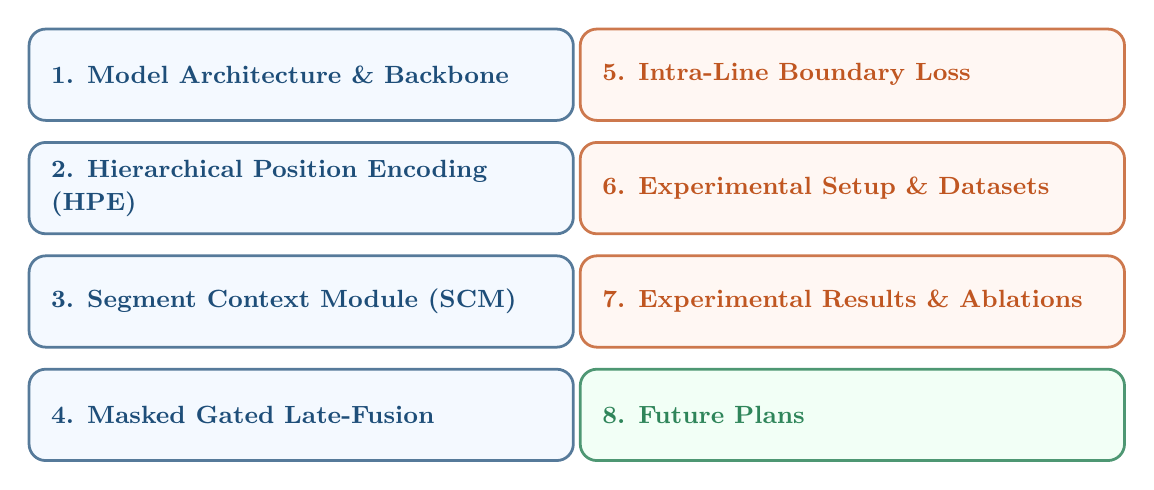
\begin{tikzpicture}[
      tocbase/.style={rounded corners=6pt, line width=1pt, inner ysep=6pt, inner xsep=8pt, text width=6.35cm, minimum width=6.65cm, minimum height=1.16cm, align=flush left, font=\fontsize{9.3pt}{12pt}\selectfont\bfseries},
      secbox1/.style={tocbase, draw=PrimaryBlue!75, fill=LightBlue!55, text=PrimaryBlue},
      secbox2/.style={tocbase, draw=PrimaryOrange!80, fill=LightOrange!80, text=PrimaryOrange},
      secbox3/.style={tocbase, draw=SuccessGreen!85, fill=LightGreen!85, text=SuccessGreen}
    ]
      % Left Column (x = -3.50cm)
      \node[secbox1] (s1) at (-3.50,  2.16) {1. Model Architecture \& Backbone};
      \node[secbox1] (s2) at (-3.50,  0.72) {2. Hierarchical Position Encoding (HPE)};
      \node[secbox1] (s3) at (-3.50, -0.72) {3. Segment Context Module (SCM)};
      \node[secbox1] (s4) at (-3.50, -2.16) {4. Masked Gated Late-Fusion};

      % Right Column (x = 3.50cm)
      \node[secbox2] (s5) at (3.50,  2.16) {5. Intra-Line Boundary Loss};
      \node[secbox2] (s6) at (3.50,  0.72) {6. Experimental Setup \& Datasets};
      \node[secbox2] (s7) at (3.50, -0.72) {7. Experimental Results \& Ablations};
      \node[secbox3] (s8) at (3.50, -2.16) {8. Future Plans};
    \end{tikzpicture}
  \end{center}
\end{frame}

% ============================================================================
% SLIDE 3: END-TO-END MODEL ARCHITECTURE DIAGRAM
% ============================================================================
\begin{frame}{1. End-to-End Model Architecture}
  \vspace{-0.1cm}
  \begin{center}
    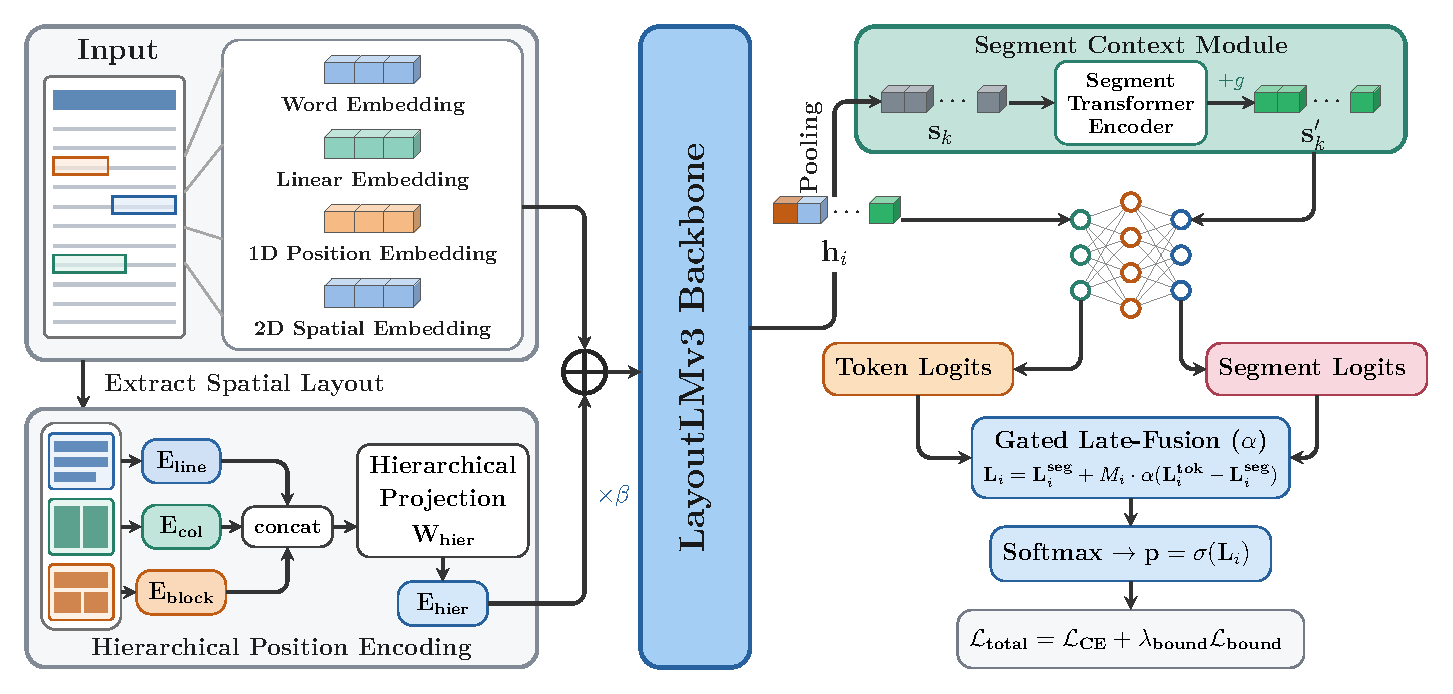
\includegraphics[width=0.95\textwidth,height=0.82\textheight,keepaspectratio]{../figures/model_architecture_heads_style.pdf}
  \end{center}
\end{frame}

% ============================================================================
% SLIDE 4: LAYOUTLMV3 BACKBONE OVERVIEW (VISUAL SHAPE FLOW)
% ============================================================================
\begin{frame}{1. LayoutLMv3 Backbone Overview}
  \vspace{0.1cm}
  \begin{center}
    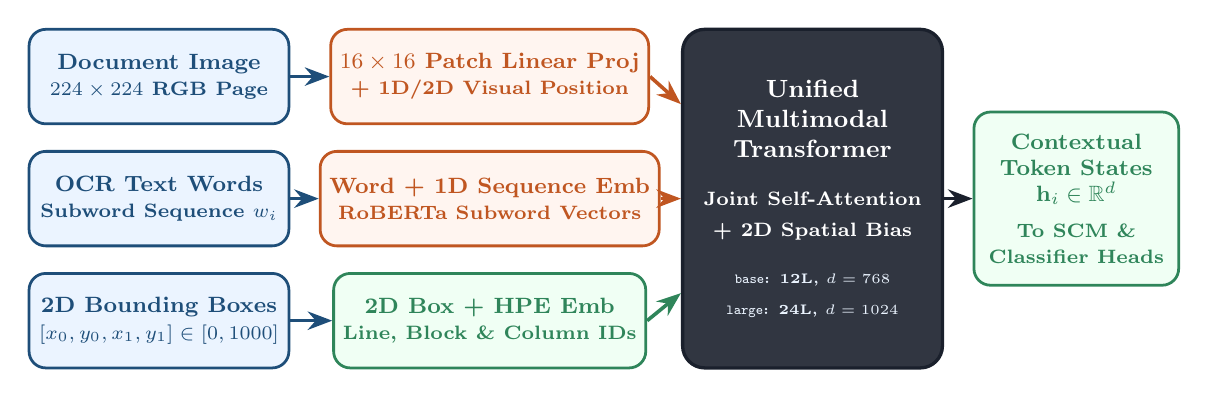
\begin{tikzpicture}[
      node distance=0.45cm,
      inp/.style={draw=PrimaryBlue, fill=LightBlue, rounded corners=6pt, line width=1pt, minimum width=3.3cm, minimum height=1.2cm, align=center, font=\footnotesize\bfseries\color{PrimaryBlue}},
      emb/.style={draw=PrimaryOrange, fill=LightOrange, rounded corners=6pt, line width=1pt, minimum width=3.5cm, minimum height=1.2cm, align=center, font=\footnotesize\bfseries\color{PrimaryOrange}},
      core/.style={draw=DarkSlate, fill=DarkSlate!90, rounded corners=8pt, line width=1.2pt, minimum width=3.3cm, minimum height=4.3cm, align=center, font=\small\bfseries\color{white}},
      outb/.style={draw=SuccessGreen, fill=LightGreen, rounded corners=6pt, line width=1pt, minimum width=2.6cm, minimum height=2.2cm, align=center, font=\footnotesize\bfseries\color{SuccessGreen}},
      arr/.style={-Stealth, line width=1.3pt, rounded corners=5pt}
    ]
      % Column 1: Raw Document Inputs
      \node[inp] (img) at (0, 1.55) {Document Image\\{\scriptsize $224 \times 224$ RGB Page}};
      \node[inp] (txt) at (0, 0) {OCR Text Words\\{\scriptsize Subword Sequence $w_i$}};
      \node[inp] (box) at (0, -1.55) {2D Bounding Boxes\\{\scriptsize $[x_0, y_0, x_1, y_1] \in [0,1000]$}};

      % Column 2: Modality Embeddings
      \node[emb] (vemb) at (4.2, 1.55) {$16\times 16$ Patch Linear Proj\\{\scriptsize + 1D/2D Visual Position}};
      \node[emb] (temb) at (4.2, 0) {Word + 1D Sequence Emb\\{\scriptsize RoBERTa Subword Vectors}};
      \node[emb, draw=SuccessGreen, fill=LightGreen, text=SuccessGreen] (hemb) at (4.2, -1.55) {2D Box + \textbf{HPE} Emb\\{\scriptsize Line, Block \& Column IDs}};

      % Column 3: Unified Backbone
      \node[core] (tr) at (8.3, 0) {Unified\\Multimodal\\Transformer\\[0.22cm]{\scriptsize Joint Self-Attention}\\{\scriptsize + 2D Spatial Bias}\\[0.22cm]{\tiny\color{LightBlue} \texttt{base}: 12L, $d=768$}\\{\tiny\color{LightBlue} \texttt{large}: 24L, $d=1024$}};

      % Column 4: Output
      \node[outb] (hi) at (11.65, 0) {Contextual\\Token States\\$\mathbf{h}_i \in \mathbb{R}^d$\\[0.12cm]{\scriptsize To SCM \&}\\{\scriptsize Classifier Heads}};

      % Connectors
      \draw[arr, PrimaryBlue] (img) -- (vemb);
      \draw[arr, PrimaryBlue] (txt) -- (temb);
      \draw[arr, PrimaryBlue] (box) -- (hemb);

      \draw[arr, PrimaryOrange] (vemb.east) -- ($(tr.west)+(0,1.2)$);
      \draw[arr, PrimaryOrange] (temb.east) -- (tr.west);
      \draw[arr, SuccessGreen] (hemb.east) -- ($(tr.west)+(0,-1.2)$);

      \draw[arr, DarkSlate] (tr.east) -- (hi.west);
    \end{tikzpicture}
  \end{center}
\end{frame}

% ============================================================================
% SLIDE 5: BACKBONE LIMITATIONS & PROPOSED SOLUTIONS (WITH REAL-LIFE EXAMPLE)
% ============================================================================
\begin{frame}{1. Backbone Limitations \& Proposed Solutions}
  \vspace{-0.15cm}
  \begin{center}
    \renewcommand{\arraystretch}{1.22}
    \setlength{\tabcolsep}{4.5pt}
    \footnotesize
    \begin{tabular}{|>{\bfseries\color{PrimaryOrange}}L{2.2cm}|L{3.6cm}|L{3.9cm}|>{\bfseries\color{PrimaryBlue}}L{3.8cm}|}
      \hline
      \rowcolor{PrimaryBlue!12}
      \textbf{\color{PrimaryBlue}Limitation} & \textbf{\color{PrimaryBlue}Failure Behavior} & \textbf{\color{PrimaryBlue}Real-Life Example} & \textbf{\color{PrimaryBlue}Proposed Solution} \\ \hline
      1. Flat 2D Coords & Raw $[x_0, y_0, x_1, y_1]$ lacks line, column, and block IDs. & Two-column fax row:\newline \texttt{FAX: (336)... | PHONE: ...} & \textbf{Hierarchical Position Encoding}\newline (Line, Block, Column IDs) \\ \hline
      \rowcolor{SoftGray}
      2. Mid-Span Noise & Multi-word entities fracture mid-line into noisy BIO tags. & Multi-word sender field:\newline \texttt{June Flynn for Eric Brown/...} & \textbf{Segment Context Module}\newline (Mean Pool + ReZero Gate) \\ \hline
      3. Segment Drift & Pure segment pooling overwrites subword boundaries. & Receipt total line:\newline \texttt{TOTAL (Qty 2.00) 60.000} & \textbf{Masked Gated Late-Fusion}\newline (Anchor Lock + Subword Gate) \\ \hline
      \rowcolor{SoftGray}
      4. Span Merging & Adjacent key--value entities on one line merge together. & Form row on one line:\newline \texttt{TO: George Baroody} & \textbf{Intra-Line Boundary Loss}\newline (Adjacent Token Pair BCE) \\ \hline
    \end{tabular}
  \end{center}
\end{frame}

% ============================================================================
% SLIDE 6: MODULE 1 (HPE) - VISUAL CONCEPT & REAL-LIFE DOCUMENT EXAMPLE
% ============================================================================
\begin{frame}{2. Hierarchical Position Encoding (HPE) -- Visual Grouping}
  \vspace{-0.1cm}
  \begin{columns}[c,totalwidth=0.97\textwidth]
    % Left: Cropped Real-Life FUNSD Form
    \begin{column}{0.54\textwidth}
      \begin{center}
        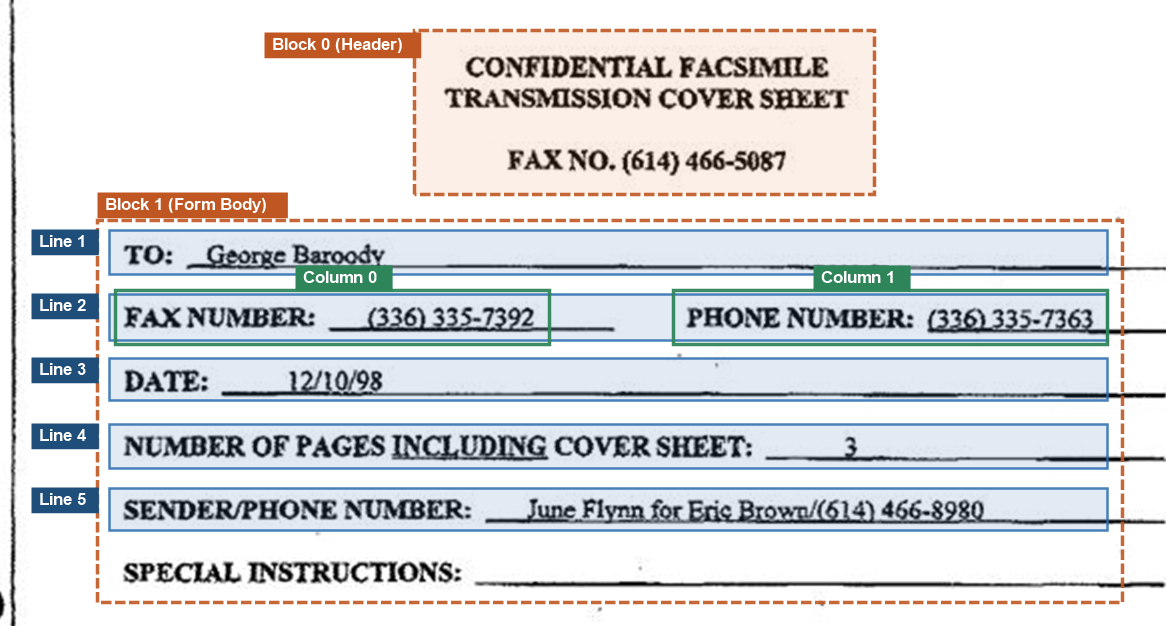
\includegraphics[width=\textwidth,height=0.76\textheight,keepaspectratio]{images/crop_hpe.png}
      \end{center}
    \end{column}

    % Right: Visual Shape Explanation of the 3 Levels
    \begin{column}{0.41\textwidth}
      \begin{center}
        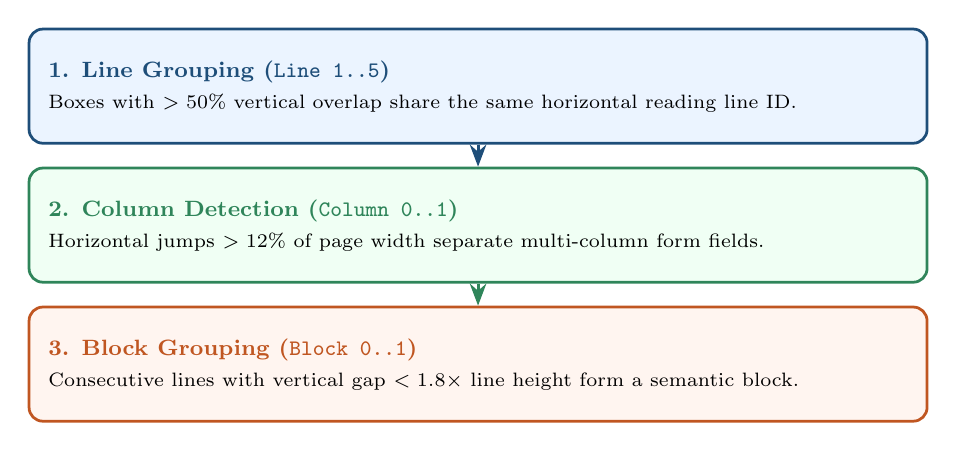
\begin{tikzpicture}[
          node distance=0.28cm,
          card/.style={rounded corners=5pt, line width=1pt, inner sep=7pt, text width=0.90\textwidth, minimum height=1.45cm, align=flush left, font=\footnotesize}
        ]
          \node[card, draw=PrimaryBlue, fill=LightBlue] (lbox) {
            \textbf{\color{PrimaryBlue}1. Line Grouping (\texttt{Line 1..5})}\\[0.06cm]
            {\scriptsize Boxes with $>50\%$ vertical overlap share the same horizontal reading line ID.}
          };
          \node[card, draw=SuccessGreen, fill=LightGreen, below=of lbox] (cbox) {
            \textbf{\color{SuccessGreen}2. Column Detection (\texttt{Column 0..1})}\\[0.06cm]
            {\scriptsize Horizontal jumps $>12\%$ of page width separate multi-column form fields.}
          };
          \node[card, draw=PrimaryOrange, fill=LightOrange, below=of cbox] (bbox) {
            \textbf{\color{PrimaryOrange}3. Block Grouping (\texttt{Block 0..1})}\\[0.06cm]
            {\scriptsize Consecutive lines with vertical gap $<1.8\times$ line height form a semantic block.}
          };
          \draw[-Stealth, line width=1.1pt, PrimaryBlue] (lbox) -- (cbox);
          \draw[-Stealth, line width=1.1pt, SuccessGreen] (cbox) -- (bbox);
        \end{tikzpicture}
      \end{center}
    \end{column}
  \end{columns}
\end{frame}

% ============================================================================
% SLIDE 7: MODULE 1 (HPE) - CORE FUNCTION & DARK-MODE CODE
% ============================================================================
\begin{frame}[fragile]{2. Hierarchical Position Encoding (HPE) -- Core Implementation}
  \vspace{-0.05cm}
  \begin{columns}[c,totalwidth=0.97\textwidth]
    % Left: Shape Diagram of Core Function
    \begin{column}{0.43\textwidth}
      \begin{center}
        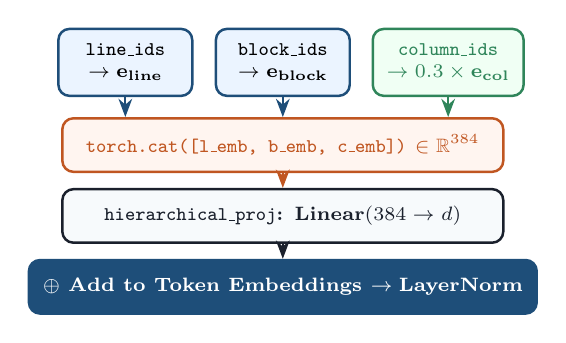
\begin{tikzpicture}[
          node distance=0.28cm,
          sbox/.style={draw=PrimaryBlue, fill=LightBlue, rounded corners=4pt, line width=0.9pt, inner sep=5pt, minimum height=0.85cm, font=\scriptsize\bfseries, align=center}
        ]
          \node[sbox, minimum width=1.7cm] (lid) at (0,0) {\texttt{line\_ids}\\$\to \mathbf{e}_{\text{line}}$};
          \node[sbox, minimum width=1.7cm] (bid) at (2.0,0) {\texttt{block\_ids}\\$\to \mathbf{e}_{\text{block}}$};
          \node[sbox, draw=SuccessGreen, fill=LightGreen, text=SuccessGreen, minimum width=1.9cm] (cid) at (4.1,0) {\texttt{column\_ids}\\$\to 0.3\times \mathbf{e}_{\text{col}}$};

          \node[sbox, draw=PrimaryOrange, fill=LightOrange, text=PrimaryOrange, minimum width=5.6cm, minimum height=0.68cm] (cat) at (2.0,-1.05) {\texttt{torch.cat([l\_emb, b\_emb, c\_emb])} $\in \mathbb{R}^{384}$};
          \node[sbox, draw=DarkSlate, fill=SoftGray, text=DarkSlate, minimum width=5.6cm, minimum height=0.68cm] (proj) at (2.0,-1.95) {\texttt{hierarchical\_proj}: $\text{Linear}(384 \to d)$};
          \node[sbox, draw=PrimaryBlue, fill=PrimaryBlue, text=white, minimum width=5.6cm, minimum height=0.68cm] (add) at (2.0,-2.85) {$\oplus$ Add to Token Embeddings $\to \text{LayerNorm}$};

          \draw[-Stealth, thick, PrimaryBlue] (lid.south) -- (lid.south |- cat.north);
          \draw[-Stealth, thick, PrimaryBlue] (bid.south) -- (bid.south |- cat.north);
          \draw[-Stealth, thick, SuccessGreen] (cid.south) -- (cid.south |- cat.north);
          \draw[-Stealth, thick, PrimaryOrange] (cat) -- (proj);
          \draw[-Stealth, thick, DarkSlate] (proj) -- (add);
        \end{tikzpicture}
      \end{center}
    \end{column}

    % Right: Concise Dark-Mode Code Block (Borderless Solid Background)
    \begin{column}{0.53\textwidth}
      {\scriptsize\bfseries\color{PrimaryBlue} \texttt{LayoutLMv3Embeddings.forward} (\texttt{modeling\_layoutlmv3.py}):}\\[0.08cm]
      \begin{tikzpicture}
        \node[fill=CodeDarkBg, draw=none, rounded corners=6pt, inner sep=7pt, text width=0.91\textwidth] {
\begin{lstlisting}[style=pydark]
def forward(
    self, input_ids: Tensor, bbox: Tensor,
    line_ids: Optional[Tensor],
    block_ids: Optional[Tensor],
    column_ids: Optional[Tensor], ...
) -> Tensor:
    ...
    l_emb = self.line_position_embeddings(line_ids)
    b_emb = self.block_position_embeddings(block_ids)
    c_emb = self.column_position_embeddings(column_ids) * 0.3
    concat_emb = torch.cat([l_emb, b_emb, c_emb], dim=-1)
    embeddings = embeddings + self.hierarchical_proj(
        concat_emb)
    return self.dropout(self.LayerNorm(embeddings))
\end{lstlisting}
        };
      \end{tikzpicture}
    \end{column}
  \end{columns}
\end{frame}

% ============================================================================
% SLIDE 8: MODULE 2 (SCM) - VISUAL CONCEPT & REAL-LIFE DOCUMENT EXAMPLE
% ============================================================================
\begin{frame}{3. Segment Context Module (SCM) -- Visual Concept}
  \vspace{-0.1cm}
  \begin{center}
    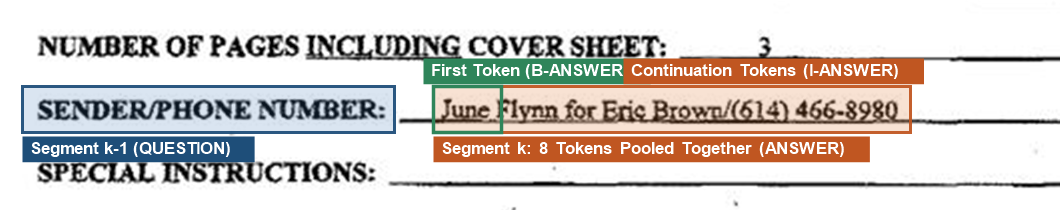
\includegraphics[width=0.90\textwidth,height=0.36\textheight,keepaspectratio]{images/crop_scm.png}
  \end{center}
  \vspace{-0.15cm}
  \begin{center}
    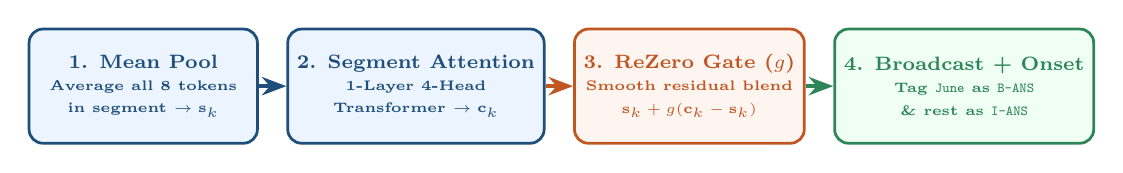
\begin{tikzpicture}[
      node distance=0.35cm,
      stage/.style={draw=PrimaryBlue, fill=LightBlue, rounded corners=5pt, line width=1pt, minimum width=2.9cm, minimum height=1.45cm, align=center, font=\scriptsize\bfseries\color{PrimaryBlue}},
      arr/.style={-Stealth, line width=1.3pt, PrimaryBlue}
    ]
      \node[stage] (s1) {1. Mean Pool\\{\tiny Average all 8 tokens}\\{\tiny in segment $\to \mathbf{s}_k$}};
      \node[stage, right=of s1] (s2) {2. Segment Attention\\{\tiny 1-Layer 4-Head}\\{\tiny Transformer $\to \mathbf{c}_k$}};
      \node[stage, draw=PrimaryOrange, fill=LightOrange, text=PrimaryOrange, right=of s2] (s3) {3. ReZero Gate ($g$)\\{\tiny Smooth residual blend}\\{\tiny $\mathbf{s}_k + g(\mathbf{c}_k - \mathbf{s}_k)$}};
      \node[stage, draw=SuccessGreen, fill=LightGreen, text=SuccessGreen, right=of s3] (s4) {4. Broadcast + Onset\\{\tiny Tag \texttt{June} as \texttt{B-ANS}}\\{\tiny \& rest as \texttt{I-ANS}}};

      \draw[arr] (s1) -- (s2);
      \draw[arr, PrimaryOrange] (s2) -- (s3);
      \draw[arr, SuccessGreen] (s3) -- (s4);
    \end{tikzpicture}
  \end{center}
\end{frame}

% ============================================================================
% SLIDE 9: MODULE 2 (SCM) - CORE FUNCTION & DARK-MODE CODE
% ============================================================================
\begin{frame}[fragile]{3. Segment Context Module (SCM) -- Core Implementation}
  \vspace{-0.05cm}
  \begin{columns}[c,totalwidth=0.97\textwidth]
    % Left: Shape Visualization of _segment_pool_and_contextualize
    \begin{column}{0.43\textwidth}
      \begin{center}
        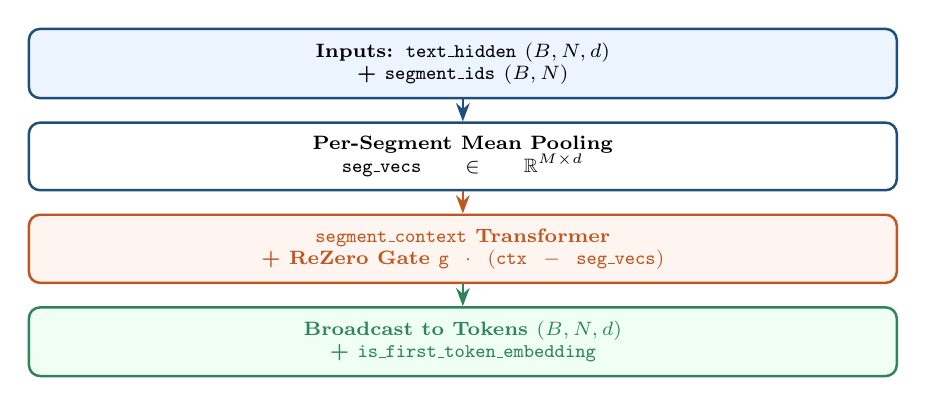
\begin{tikzpicture}[
          node distance=0.28cm,
          fbox/.style={draw=PrimaryBlue, fill=LightBlue, rounded corners=4pt, line width=0.9pt, inner sep=5pt, text width=0.88\textwidth, minimum height=0.82cm, align=center, font=\scriptsize\bfseries}
        ]
          \node[fbox] (in) {Inputs: \texttt{text\_hidden} $(B, N, d)$\\+ \texttt{segment\_ids} $(B, N)$};
          \node[fbox, fill=white, below=of in] (pool) {Per-Segment Mean Pooling\\$\texttt{seg\_vecs} \in \mathbb{R}^{M \times d}$};
          \node[fbox, draw=PrimaryOrange, fill=LightOrange, text=PrimaryOrange, below=of pool] (tr) {\texttt{segment\_context} Transformer\\+ ReZero Gate $\texttt{g} \cdot (\texttt{ctx} - \texttt{seg\_vecs})$};
          \node[fbox, draw=SuccessGreen, fill=LightGreen, text=SuccessGreen, below=of tr] (out) {Broadcast to Tokens $(B, N, d)$\\+ \texttt{is\_first\_token\_embedding}};

          \draw[-Stealth, thick, PrimaryBlue] (in) -- (pool);
          \draw[-Stealth, thick, PrimaryOrange] (pool) -- (tr);
          \draw[-Stealth, thick, SuccessGreen] (tr) -- (out);
        \end{tikzpicture}
      \end{center}
    \end{column}

    % Right: Concise Dark-Mode Code (Borderless Solid Background)
    \begin{column}{0.53\textwidth}
      {\scriptsize\bfseries\color{PrimaryBlue} \texttt{\_segment\_pool\_and\_contextualize} (\texttt{modeling\_layoutlmv3\_segment.py}):}\\[0.08cm]
      \begin{tikzpicture}
        \node[fill=CodeDarkBg, draw=none, rounded corners=6pt, inner sep=7pt, text width=0.91\textwidth] {
\begin{lstlisting}[style=pydark]
def _segment_pool_and_contextualize(
    self, text_hidden: Tensor, segment_ids: Tensor
) -> Tensor:
    ...
    seg_vecs = torch.stack([
        text_hidden[b, seg_b == sid].mean(dim=0)
        for sid in unique_segs], dim=0)
    ctx = self.segment_context(
        seg_vecs.unsqueeze(0)).squeeze(0)
    seg_vecs = seg_vecs + self.segment_context_gate * (
        ctx - seg_vecs)
    ...
    is_first[:, 1:] = (
        segment_ids[:, 1:] != segment_ids[:, :-1]).long()
    return seg_repr + self.is_first_token_embedding(is_first)
\end{lstlisting}
        };
      \end{tikzpicture}
    \end{column}
  \end{columns}
\end{frame}

% ============================================================================
% SLIDE 10: MODULE 3 (LATE-FUSION) - VISUAL CONCEPT & REAL-LIFE EXAMPLE
% ============================================================================
\begin{frame}{4. Masked Gated Late-Fusion -- Visual Concept}
  \vspace{-0.05cm}
  \begin{columns}[c,totalwidth=0.97\textwidth]
    % Left: Cropped Real-Life CORD Receipt
    \begin{column}{0.48\textwidth}
      \begin{center}
        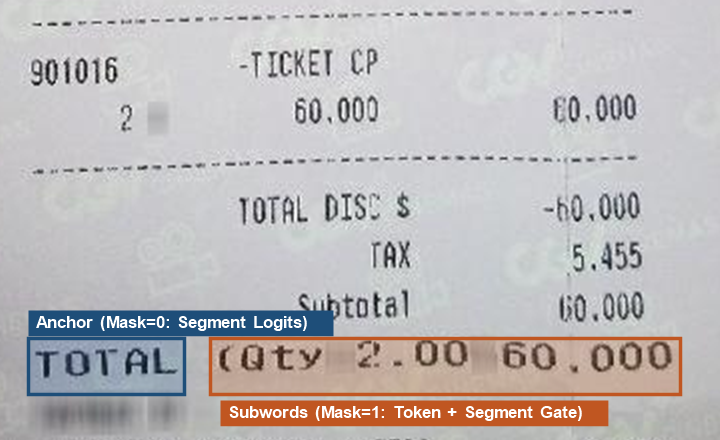
\includegraphics[width=\textwidth,height=0.74\textheight,keepaspectratio]{images/crop_fusion.png}
      \end{center}
    \end{column}

    % Right: Shape Router Diagram
    \begin{column}{0.47\textwidth}
      \begin{center}
        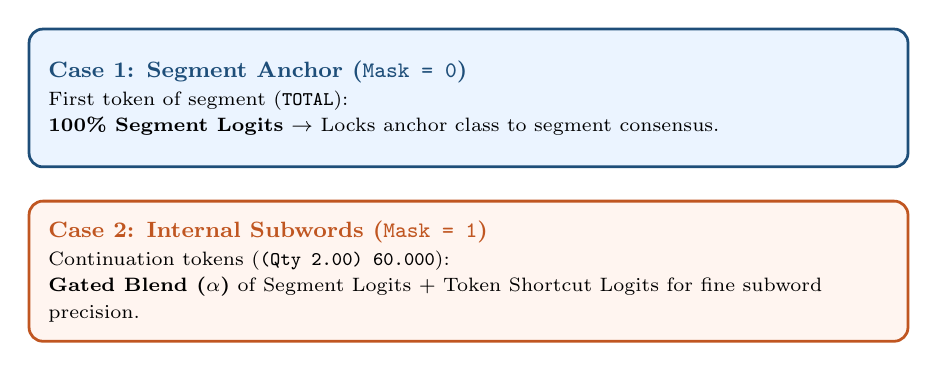
\begin{tikzpicture}[
          node distance=0.35cm,
          rbox/.style={rounded corners=5pt, line width=1pt, inner sep=7pt, text width=0.88\textwidth, minimum height=1.75cm, align=flush left, font=\footnotesize}
        ]
          \node[rbox, draw=PrimaryBlue, fill=LightBlue] (m0) {
            \textbf{\color{PrimaryBlue}Case 1: Segment Anchor (\texttt{Mask = 0})}\\[0.08cm]
            {\scriptsize First token of segment (\texttt{TOTAL}):\\
            \textbf{100\% Segment Logits} $\to$ Locks anchor class to segment consensus.}
          };
          \node[rbox, draw=PrimaryOrange, fill=LightOrange, below=0.4cm of m0] (m1) {
            \textbf{\color{PrimaryOrange}Case 2: Internal Subwords (\texttt{Mask = 1})}\\[0.08cm]
            {\scriptsize Continuation tokens (\texttt{(Qty 2.00) 60.000}):\\
            \textbf{Gated Blend ($\alpha$)} of Segment Logits + Token Shortcut Logits for fine subword precision.}
          };
        \end{tikzpicture}
      \end{center}
    \end{column}
  \end{columns}
\end{frame}

% ============================================================================
% SLIDE 11: MODULE 3 (LATE-FUSION) - CORE FUNCTION & DARK-MODE CODE
% ============================================================================
\begin{frame}[fragile]{4. Masked Gated Late-Fusion -- Core Implementation}
  \vspace{-0.05cm}
  \begin{columns}[c,totalwidth=0.97\textwidth]
    % Left: Shape Gate Circuit
    \begin{column}{0.43\textwidth}
      \begin{center}
        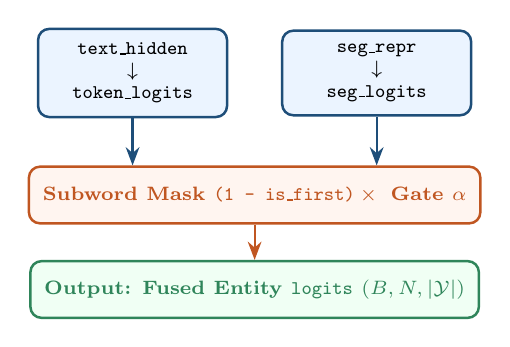
\begin{tikzpicture}[
          cbox/.style={draw=PrimaryBlue, fill=LightBlue, rounded corners=4pt, line width=0.9pt, inner sep=5pt, minimum height=0.85cm, font=\scriptsize\bfseries, align=center}
        ]
          \node[cbox, minimum width=2.4cm] (th) at (0,0) {\texttt{text\_hidden}\\$\downarrow$\\$\texttt{token\_logits}$};
          \node[cbox, minimum width=2.4cm] (sr) at (3.1,0) {\texttt{seg\_repr}\\$\downarrow$\\$\texttt{seg\_logits}$};
          \node[cbox, draw=PrimaryOrange, fill=LightOrange, text=PrimaryOrange, minimum width=5.5cm, minimum height=0.72cm] (gate) at (1.55,-1.55) {Subword Mask $\texttt{(1 - is\_first)} \times \text{ Gate } \alpha$};
          \node[cbox, draw=SuccessGreen, fill=LightGreen, text=SuccessGreen, minimum width=5.5cm, minimum height=0.72cm] (out) at (1.55,-2.75) {Output: Fused Entity \texttt{logits} $(B, N, |\mathcal{Y}|)$};

          \draw[-Stealth, thick, PrimaryBlue] (th) -- (th |- gate.north);
          \draw[-Stealth, thick, PrimaryBlue] (sr) -- (sr |- gate.north);
          \draw[-Stealth, thick, PrimaryOrange] (gate) -- (out);
        \end{tikzpicture}
      \end{center}
    \end{column}

    % Right: Concise Dark-Mode Code (Borderless Solid Background)
    \begin{column}{0.53\textwidth}
      {\scriptsize\bfseries\color{PrimaryBlue} \texttt{LayoutLMv3ForSegmentTokenClassification.forward}:}\\[0.08cm]
      \begin{tikzpicture}
        \node[fill=CodeDarkBg, draw=none, rounded corners=6pt, inner sep=7pt, text width=0.91\textwidth] {
\begin{lstlisting}[style=pydark]
def forward(
    self, input_ids: Tensor, bbox: Tensor,
    segment_ids: Tensor, ...
) -> TokenClassifierOutput:
    ...
    token_logits = self.token_classifier(
        self.dropout(text_hidden))
    seg_logits = self.classifier(self.dropout(seg_repr))

    subword_mask = (1 - is_first).unsqueeze(-1).float()
    alpha = self.alpha_max * torch.sigmoid(self.fusion_gate)
    logits = seg_logits + subword_mask * alpha * (
        token_logits - seg_logits)
    ...
\end{lstlisting}
        };
      \end{tikzpicture}
    \end{column}
  \end{columns}
\end{frame}

% ============================================================================
% SLIDE 12: MODULE 4 (BOUNDARY LOSS) - VISUAL CONCEPT & REAL-LIFE EXAMPLE
% ============================================================================
\begin{frame}{5. Intra-Line Boundary Loss -- Visual Concept}
  \vspace{-0.05cm}
  \begin{columns}[c,totalwidth=0.97\textwidth]
    % Left: Cropped Real-Life FUNSD Intra-Line Transitions
    \begin{column}{0.54\textwidth}
      \begin{center}
        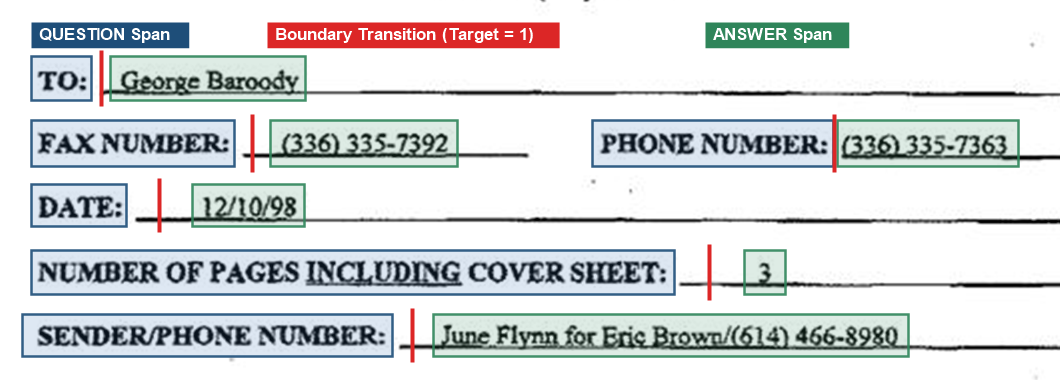
\includegraphics[width=\textwidth,height=0.74\textheight,keepaspectratio]{images/crop_boundary.png}
      \end{center}
    \end{column}

    % Right: Visual Shape Pair Comparison
    \begin{column}{0.41\textwidth}
      \begin{center}
        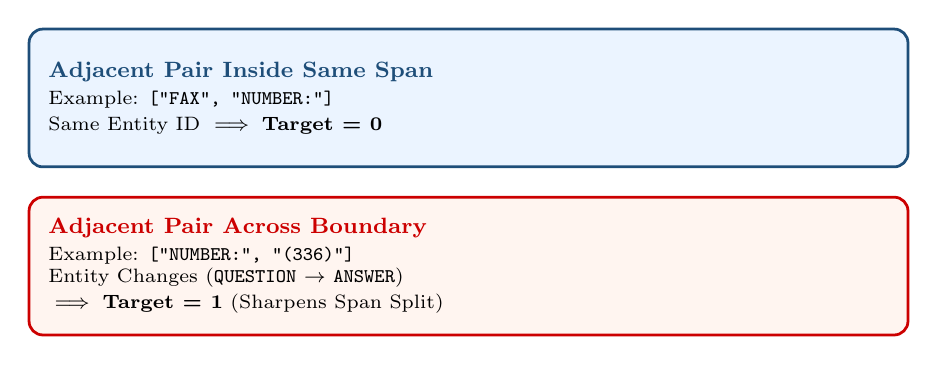
\begin{tikzpicture}[
          node distance=0.3cm,
          bbox/.style={rounded corners=5pt, line width=1pt, inner sep=7pt, text width=0.88\textwidth, minimum height=1.75cm, align=flush left, font=\footnotesize}
        ]
          \node[bbox, draw=PrimaryBlue, fill=LightBlue] (b0) {
            \textbf{\color{PrimaryBlue}Adjacent Pair Inside Same Span}\\[0.06cm]
            {\scriptsize Example: \texttt{["FAX", "NUMBER:"]}\\
            Same Entity ID $\implies \textbf{Target = 0}$}
          };
          \node[bbox, draw= red!80!black, fill=LightOrange, below=0.35cm of b0] (b1) {
            \textbf{\color{red!80!black}Adjacent Pair Across Boundary}\\[0.06cm]
            {\scriptsize Example: \texttt{["NUMBER:", "(336)"]}\\
            Entity Changes (\texttt{QUESTION} $\to$ \texttt{ANSWER})\\
            $\implies \textbf{Target = 1}$ (Sharpens Span Split)}
          };
        \end{tikzpicture}
      \end{center}
    \end{column}
  \end{columns}
\end{frame}

% ============================================================================
% SLIDE 13: MODULE 4 (BOUNDARY LOSS) - CORE FUNCTION & DARK-MODE CODE
% ============================================================================
\begin{frame}[fragile]{5. Intra-Line Boundary Loss -- Core Implementation}
  \vspace{-0.05cm}
  \begin{columns}[c,totalwidth=0.97\textwidth]
    % Left: Shape Diagram of _compute_boundary_loss
    \begin{column}{0.43\textwidth}
      \begin{center}
        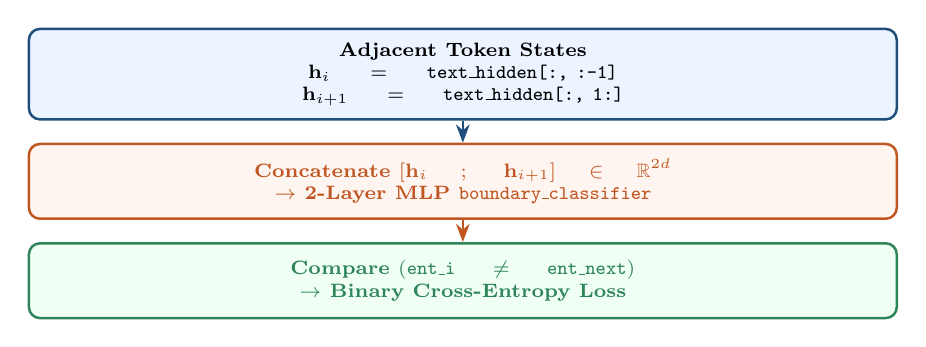
\begin{tikzpicture}[
          node distance=0.28cm,
          bbox/.style={draw=PrimaryBlue, fill=LightBlue, rounded corners=4pt, line width=0.9pt, inner sep=5pt, text width=0.88\textwidth, minimum height=0.95cm, align=center, font=\scriptsize\bfseries}
        ]
          \node[bbox] (p1) {Adjacent Token States\\$\mathbf{h}_i = \texttt{text\_hidden[:, :-1]}$\\$\mathbf{h}_{i+1} = \texttt{text\_hidden[:, 1:]}$};
          \node[bbox, draw=PrimaryOrange, fill=LightOrange, text=PrimaryOrange, below=of p1] (p2) {Concatenate $[\mathbf{h}_i \;;\; \mathbf{h}_{i+1}] \in \mathbb{R}^{2d}$\\$\to$ 2-Layer MLP \texttt{boundary\_classifier}};
          \node[bbox, draw=SuccessGreen, fill=LightGreen, text=SuccessGreen, below=of p2] (p3) {Compare $(\texttt{ent\_i} \neq \texttt{ent\_next})$\\$\to$ Binary Cross-Entropy Loss};

          \draw[-Stealth, thick, PrimaryBlue] (p1) -- (p2);
          \draw[-Stealth, thick, PrimaryOrange] (p2) -- (p3);
        \end{tikzpicture}
      \end{center}
    \end{column}

    % Right: Concise Dark-Mode Code (Borderless Solid Background)
    \begin{column}{0.53\textwidth}
      {\scriptsize\bfseries\color{PrimaryBlue} \texttt{\_compute\_boundary\_loss} (\texttt{modeling\_layoutlmv3\_segment.py}):}\\[0.08cm]
      \begin{tikzpicture}
        \node[fill=CodeDarkBg, draw=none, rounded corners=6pt, inner sep=7pt, text width=0.91\textwidth] {
\begin{lstlisting}[style=pydark]
def _compute_boundary_loss(
    self, text_hidden: Tensor,
    entity_ids: Tensor, labels: Tensor
) -> Tensor:
    h_pair = torch.cat([
        text_hidden[:, :-1, :],
        text_hidden[:, 1:, :]], dim=-1)
    b_logits = self.boundary_classifier(h_pair).squeeze(-1)
    ...
    b_labels = (
        entity_ids[:, :-1] != entity_ids[:, 1:]).float()
    return F.binary_cross_entropy_with_logits(
        b_logits[valid], b_labels[valid])
\end{lstlisting}
        };
      \end{tikzpicture}
    \end{column}
  \end{columns}
\end{frame}

% ============================================================================
% SLIDE 14: EXPERIMENTAL SETUP - HARDWARE, ENVIRONMENT & DATASETS
% ============================================================================
\begin{frame}{6. Experimental Setup: Hardware, Environment \& Datasets}
  \vspace{0.05cm}
  \begin{center}
    \begin{tikzpicture}
      % Left Card: Training Environment
      \node[draw=PrimaryBlue, fill=PrimaryBlue!6, rounded corners=6pt, line width=0.9pt, inner sep=7pt, text width=6.1cm, minimum height=5.15cm, align=flush center] (envcard) at (-3.32, 0) {
        {\small\bfseries\color{PrimaryBlue} Training Environment}\\[0.14cm]
        \renewcommand{\arraystretch}{1.28}
        \setlength{\tabcolsep}{3pt}
        \scriptsize
        \begin{tabular}{|>{\bfseries}L{1.85cm}|L{3.75cm}|}
          \hline
          GPU Server & \textbf{NVIDIA A100-SXM4-80GB} \\ \hline
          System RAM & 167 GiB Host Memory \\ \hline
          Environment & Ubuntu Linux, Python 3.7.16 \\ \hline
          DL Stack & PyTorch 1.10.0+cu111, FP16 \\ \hline
          Backbone Lib & Transformers 4.12.5 \\ \hline
          Metric Lib & \texttt{seqeval} 1.2.2 (Strict BIO) \\ \hline
          Random Seeds & 3 Seeds: $\{42, 123, 1993\}$ \\ \hline
        \end{tabular}
      };

      % Right Card: Benchmark Datasets
      \node[draw=PrimaryOrange, fill=PrimaryOrange!6, rounded corners=6pt, line width=0.9pt, inner sep=7pt, text width=6.1cm, minimum height=5.15cm, align=flush center] (datacard) at (3.32, 0) {
        {\small\bfseries\color{PrimaryOrange} Benchmark Datasets}\\[0.14cm]
        \renewcommand{\arraystretch}{1.38}
        \setlength{\tabcolsep}{3pt}
        \scriptsize
        \begin{tabular}{|>{\bfseries}L{1.75cm}|C{1.80cm}|C{1.85cm}|}
          \hline
          \textbf{Attribute} & \textbf{FUNSD} & \textbf{CORD} \\ \hline
          Document Type & Scanned Forms & Retail Receipts \\ \hline
          Total Images & 199 & 1,000 \\ \hline
          Train / Val & 149 / -- & 800 / 100 \\ \hline
          Test Split & 50 pages & 100 pages \\ \hline
          Entity Classes & 3 (7 BIO tags) & 30 (61 BIO tags) \\ \hline
          Layout Style & Multi-column & Tabular rows \\ \hline
        \end{tabular}
      };
    \end{tikzpicture}
  \end{center}
\end{frame}

% ============================================================================
% SLIDE 15: RUN CONFIGURATIONS & HYPERPARAMETERS (LARGE READABLE FONT)
% ============================================================================
\begin{frame}{6. Run Configurations \& Hyperparameters}
  \vspace{-0.15cm}
  \begin{center}
    \renewcommand{\arraystretch}{1.12}
    \setlength{\tabcolsep}{5pt}
    \footnotesize
    \begin{tabular}{|>{\bfseries\color{PrimaryBlue}}L{3.9cm}|C{2.15cm}|C{2.15cm}|C{2.15cm}|C{2.15cm}|}
      \hline
      \rowcolor{PrimaryBlue!15}
      \textbf{Configuration Parameter} & \textbf{FUNSD}\newline\textbf{(\texttt{base})} & \textbf{CORD}\newline\textbf{(\texttt{base})} & \textbf{FUNSD}\newline\textbf{(\texttt{large})} & \textbf{CORD}\newline\textbf{(\texttt{large})} \\ \hline
      Pretrained Checkpoint & \multicolumn{2}{c|}{\texttt{microsoft/layoutlmv3-base}} & \multicolumn{2}{c|}{\texttt{microsoft/layoutlmv3-large}} \\ \hline
      Architecture Scale & \multicolumn{2}{c|}{12 Layers, $d=768$ (125M)} & \multicolumn{2}{c|}{24 Layers, $d=1024$ (356M)} \\ \hline
      Optimizer \& Weight Decay & \multicolumn{4}{c|}{AdamW ($\beta_1 = 0.9, \beta_2 = 0.999$, Weight Decay $= 0.01$)} \\ \hline
      Training Steps \& Warmup & \multicolumn{4}{c|}{$1,000$ Steps ($10\%$ Linear Warmup $= 100$ Steps)} \\ \hline
      Backbone Learning Rate & $5 \times 10^{-5}$ & $5 \times 10^{-5}$ & $1 \times 10^{-5}$ & $5 \times 10^{-5}$ \\ \hline
      Specialized Module LR & \multicolumn{4}{c|}{$5 \times 10^{-4}$ (HPE, SCM, Late-Fusion, Boundary Classifier)} \\ \hline
      Effective Batch Size & $16$ & $64$ & $16$ & $16$ \\ \hline
      HPE Max $(N_{\text{line}}, N_{\text{block}}, N_{\text{col}})$ & $(50, 20, 10)$ & $(80, 15, 8)$ & $(50, 20, 10)$ & $(80, 15, 8)$ \\ \hline
    \end{tabular}
  \end{center}
\end{frame}

% ============================================================================
% SLIDE 16: MAIN RESULTS - BASELINE VS PROPOSED MODEL (LARGE READABLE FONT)
% ============================================================================
\begin{frame}{7. Experimental Results: Baseline vs.\ Proposed Model (3 Seeds)}
  \vspace{-0.15cm}
  \begin{columns}[c,totalwidth=0.98\textwidth]
    % Left: Large-Font Comparison Table
    \begin{column}{0.65\textwidth}
      \renewcommand{\arraystretch}{1.24}
      \setlength{\tabcolsep}{1.5pt}
      \footnotesize
      \begin{tabular}{|L{2.68cm}|C{1.15cm}|C{1.82cm}|C{1.82cm}|C{1.82cm}|}
        \hline
        \rowcolor{PrimaryBlue!15}
        \textbf{Model} & \textbf{Data} & \textbf{Prec. (\%)} & \textbf{Rec. (\%)} & \textbf{F1 (\%)} \\ \hline
        Baseline (\texttt{base}) & FUNSD & $89.32 \pm 1.31$ & $90.53 \pm 0.48$ & $89.92 \pm 0.85$ \\ \hline
        \rowcolor{LightBlue}
        \textbf{Proposed (\texttt{base})} & \textbf{FUNSD} & $\mathbf{91.82 \pm 0.05}$ & $\mathbf{91.33 \pm 0.28}$ & $\mathbf{91.58 \pm 0.16}$ \\ \hline\hline
        Baseline (\texttt{large}) & FUNSD & $90.69 \pm 1.01$ & $91.80 \pm 0.23$ & $91.24 \pm 0.62$ \\ \hline
        \rowcolor{LightBlue}
        \textbf{Proposed (\texttt{large})} & \textbf{FUNSD} & $\mathbf{92.31 \pm 0.51}$ & $\mathbf{92.60 \pm 0.10}$ & $\mathbf{92.45 \pm 0.26}$ \\ \hline\hline
        Baseline (\texttt{base}) & CORD & $96.50 \pm 0.39$ & $96.94 \pm 0.28$ & $96.72 \pm 0.33$ \\ \hline
        \rowcolor{LightOrange}
        \textbf{Proposed (\texttt{base})} & \textbf{CORD} & $\mathbf{96.80 \pm 0.27}$ & $\mathbf{97.02 \pm 0.15}$ & $\mathbf{96.91 \pm 0.21}$ \\ \hline\hline
        Baseline (\texttt{large}) & CORD & $96.96 \pm 0.30$ & $97.35 \pm 0.04$ & $97.15 \pm 0.17$ \\ \hline
        \rowcolor{LightOrange}
        \textbf{Proposed (\texttt{large})} & \textbf{CORD} & $\mathbf{97.28 \pm 0.04}$ & $\mathbf{97.43 \pm 0.04}$ & $\mathbf{97.35 \pm 0.04}$ \\ \hline
      \end{tabular}
    \end{column}

    % Right: Visual Bar Charts
    \begin{column}{0.32\textwidth}
      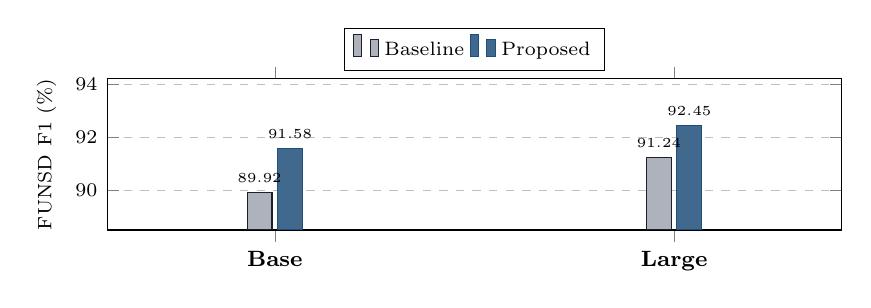
\begin{tikzpicture}
        \begin{axis}[
          ybar,
          bar width=9pt,
          enlarge x limits=0.42,
          width=0.90\textwidth,
          height=3.5cm,
          ymin=88.5, ymax=94.2,
          ylabel={\scriptsize FUNSD F1 (\%)},
          symbolic x coords={Base, Large},
          xtick=data,
          xticklabel style={font=\footnotesize\bfseries},
          yticklabel style={font=\scriptsize},
          ymajorgrids=true,
          grid style=dashed,
          legend style={at={(0.5,1.05)}, anchor=south, legend columns=2, font=\scriptsize},
          nodes near coords,
          nodes near coords style={font=\tiny\bfseries, /pgf/number format/fixed, /pgf/number format/precision=2}
        ]
          \addplot[fill=MutedGray!45, draw=DarkSlate] coordinates {(Base, 89.92) (Large, 91.24)};
          \addplot[fill=PrimaryBlue!85, draw=PrimaryBlue] coordinates {(Base, 91.58) (Large, 92.45)};
          \legend{Baseline, Proposed}
        \end{axis}
      \end{tikzpicture}

      \vspace{-0.1cm}
      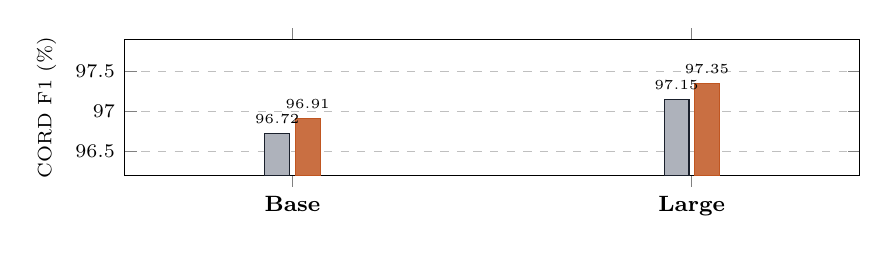
\begin{tikzpicture}
        \begin{axis}[
          ybar,
          bar width=9pt,
          enlarge x limits=0.42,
          width=0.90\textwidth,
          height=3.3cm,
          ymin=96.2, ymax=97.9,
          ylabel={\scriptsize CORD F1 (\%)},
          symbolic x coords={Base, Large},
          xtick=data,
          xticklabel style={font=\footnotesize\bfseries},
          yticklabel style={font=\scriptsize},
          ymajorgrids=true,
          grid style=dashed,
          nodes near coords,
          nodes near coords style={font=\tiny\bfseries, /pgf/number format/fixed, /pgf/number format/precision=2}
        ]
          \addplot[fill=MutedGray!45, draw=DarkSlate] coordinates {(Base, 96.72) (Large, 97.15)};
          \addplot[fill=PrimaryOrange!85, draw=PrimaryOrange] coordinates {(Base, 96.91) (Large, 97.35)};
        \end{axis}
      \end{tikzpicture}
    \end{column}
  \end{columns}
\end{frame}

% ============================================================================
% SLIDE 17: COMPONENT ABLATION STUDY (LARGE READABLE FONT & CENTERED CARDS)
% ============================================================================
\begin{frame}{7. Component Ablation Study (3-Seed Mean $\pm$ Std F1 \%)}
  \vspace{-0.18cm}
  \begin{center}
    \renewcommand{\arraystretch}{1.12}
    \setlength{\tabcolsep}{5pt}
    \footnotesize
    \begin{tabular}{|L{4.3cm}|C{2.05cm}|C{2.05cm}|C{2.05cm}|C{2.05cm}|}
      \hline
      \rowcolor{PrimaryBlue!15}
      \textbf{Ablation Configuration} & \textbf{FUNSD}\newline\textbf{(\texttt{base})} & \textbf{CORD}\newline\textbf{(\texttt{base})} & \textbf{FUNSD}\newline\textbf{(\texttt{large})} & \textbf{CORD}\newline\textbf{(\texttt{large})} \\ \hline
      1. Baseline (Vanilla LayoutLMv3) & $89.92 \pm 0.85$ & $96.72 \pm 0.33$ & $91.24 \pm 0.62$ & $97.15 \pm 0.17$ \\ \hline
      \rowcolor{LightBlue}
      \textbf{2. Full Model (HPE + SCM + Bound)} & $\mathbf{91.58 \pm 0.16}$ & $\mathbf{96.91 \pm 0.21}$ & $\mathbf{92.45 \pm 0.26}$ & $\mathbf{97.35 \pm 0.04}$ \\ \hline
      3. Ablation: \texttt{w/o Boundary Loss} & $91.62 \pm 0.19$ & $97.06 \pm 0.18$ & $92.15 \pm 0.24$ & $97.01 \pm 0.42$ \\ \hline
      4. Ablation: \texttt{w/o HPE} & $91.33 \pm 0.27$ & $97.10 \pm 0.15$ & $92.69 \pm 0.18$ & -- \\ \hline
      \rowcolor{LightOrange}
      \textbf{5. Ablation: \texttt{w/o Segment (SCM)}} & $\mathbf{90.36 \pm 0.30}$ & $\mathbf{96.59 \pm 0.57}$ & $\mathbf{91.01 \pm 0.23}$ & $\mathbf{96.84 \pm 0.13}$ \\ \hline
    \end{tabular}
  \end{center}

  \vspace{0.08cm}
  \begin{center}
    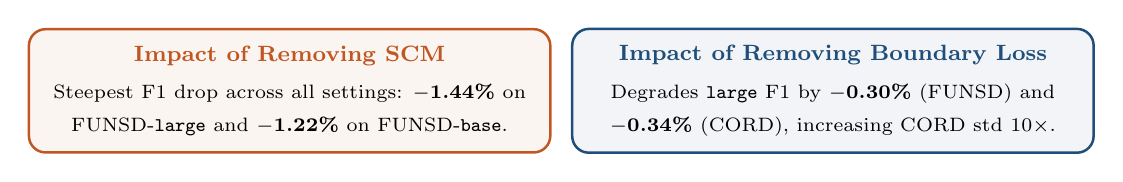
\begin{tikzpicture}
      \node[draw=PrimaryOrange, fill=PrimaryOrange!6, rounded corners=6pt, line width=0.9pt, inner sep=6pt, text width=6.2cm, minimum height=1.22cm, align=flush center] at (-3.45, 0) {
        {\footnotesize\bfseries\color{PrimaryOrange} Impact of Removing SCM}\\[0.05cm]
        {\scriptsize Steepest F1 drop across all settings: \textbf{$-$1.44\%} on FUNSD-\texttt{large} and \textbf{$-$1.22\%} on FUNSD-\texttt{base}.}
      };
      \node[draw=PrimaryBlue, fill=PrimaryBlue!6, rounded corners=6pt, line width=0.9pt, inner sep=6pt, text width=6.2cm, minimum height=1.22cm, align=flush center] at (3.45, 0) {
        {\footnotesize\bfseries\color{PrimaryBlue} Impact of Removing Boundary Loss}\\[0.05cm]
        {\scriptsize Degrades \texttt{large} F1 by \textbf{$-$0.30\%} (FUNSD) and \textbf{$-$0.34\%} (CORD), increasing CORD std $10\times$.}
      };
    \end{tikzpicture}
  \end{center}
\end{frame}

% ============================================================================
% SLIDE 18: ENTITY-LEVEL ERROR BREAKDOWN (LARGE READABLE FONT)
% ============================================================================
\begin{frame}{7. Entity-Level Error Breakdown on FUNSD ($1,998$ Test Entities)}
  \vspace{0.05cm}
  \begin{columns}[c,totalwidth=0.96\textwidth]
    \begin{column}{0.56\textwidth}
      \renewcommand{\arraystretch}{1.35}
      \setlength{\tabcolsep}{4pt}
      \footnotesize
      \begin{tabular}{|L{3.3cm}|C{1.3cm}|C{1.4cm}|C{1.2cm}|}
        \hline
        \rowcolor{PrimaryBlue!15}
        \textbf{Entity Outcome Category} & \textbf{Baseline} & \textbf{Proposed} & \textbf{Diff.} \\ \hline
        Exact Span \& Class (TP $\uparrow$) & $1,806$ & $\mathbf{1,830}$ & \textcolor{SuccessGreen}{\textbf{+24}} \\ \hline
        \rowcolor{LightGreen}
        \textbf{Span Boundary Error ($\downarrow$)} & $23$ $(19/4)$ & $\mathbf{4}$ $(4/0)$ & \textcolor{SuccessGreen}{\textbf{$-$82.6\%}} \\ \hline
        Missed Entities (FN $\downarrow$) & $79$ & $\mathbf{71}$ & \textcolor{SuccessGreen}{\textbf{$-$8}} \\ \hline
        Spurious Predictions (FP $\downarrow$) & $72$ & $\mathbf{59}$ & \textcolor{SuccessGreen}{\textbf{$-$13}} \\ \hline
      \end{tabular}
    \end{column}

    \begin{column}{0.38\textwidth}
      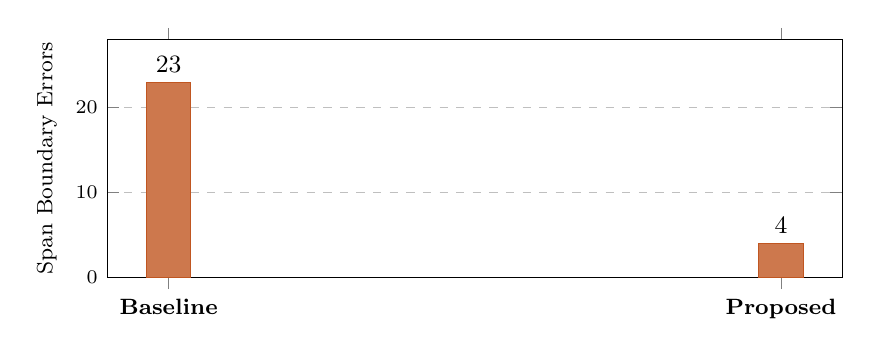
\begin{tikzpicture}
        \begin{axis}[
          ybar,
          bar width=16pt,
          width=0.90\textwidth,
          height=4.6cm,
          ymin=0, ymax=28,
          ylabel={\footnotesize Span Boundary Errors},
          symbolic x coords={Baseline, Proposed},
          xtick=data,
          xticklabel style={font=\footnotesize\bfseries},
          yticklabel style={font=\scriptsize},
          ymajorgrids=true,
          grid style=dashed,
          nodes near coords,
          nodes near coords style={font=\small\bfseries}
        ]
          \addplot[fill=PrimaryOrange!80, draw=PrimaryOrange] coordinates {(Baseline, 23) (Proposed, 4)};
        \end{axis}
      \end{tikzpicture}
    \end{column}
  \end{columns}
\end{frame}

% ============================================================================
% SLIDE 19: FUTURE PLANS (CLEAN MILESTONES, NO SUB-DESCRIPTIONS)
% ============================================================================
\begin{frame}{8. Future plans}
  \vspace{0.35cm}
  \begin{center}
    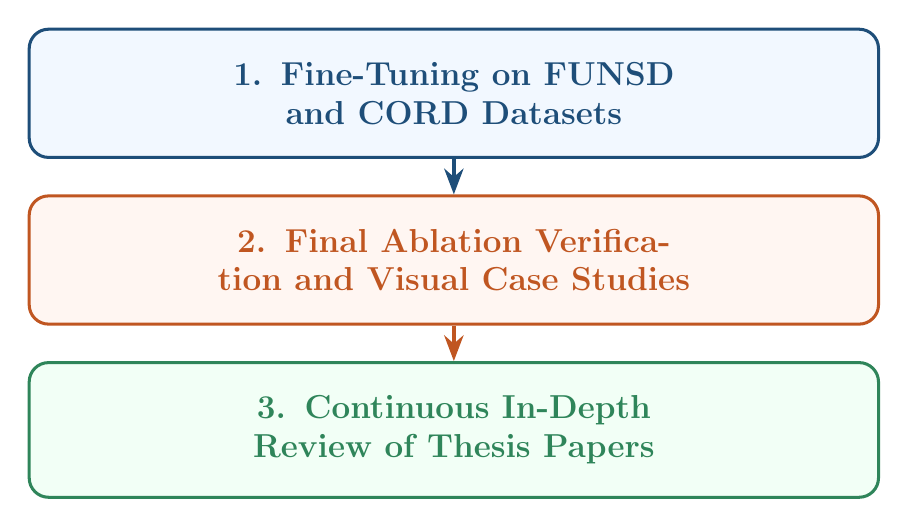
\begin{tikzpicture}[
      node distance=0.45cm,
      planbox/.style={draw=PrimaryBlue, fill=LightBlue!65, rounded corners=7pt, line width=1.1pt, inner sep=12pt, text width=0.82\textwidth, minimum height=1.15cm, align=center, font=\large\bfseries\color{PrimaryBlue}}
    ]
      \node[planbox] (p1) {1. Fine-Tuning on FUNSD and CORD Datasets};
      \node[planbox, draw=PrimaryOrange, fill=LightOrange!85, text=PrimaryOrange, below=of p1] (p2) {2. Final Ablation Verification and Visual Case Studies};
      \node[planbox, draw=SuccessGreen, fill=LightGreen!85, text=SuccessGreen, below=of p2] (p3) {3. Continuous In-Depth Review of Thesis Papers};

      \draw[-Stealth, line width=1.4pt, PrimaryBlue] (p1) -- (p2);
      \draw[-Stealth, line width=1.4pt, PrimaryOrange] (p2) -- (p3);
    \end{tikzpicture}
  \end{center}
\end{frame}

% ============================================================================
% SLIDE 20: CLOSING SLIDE (TOP-MIDDLE LOGO, CLEAN, NO REDUNDANT LABELS)
% ============================================================================
\begin{frame}[plain]
  \vspace*{0.25cm}
  \begin{center}
    
\includegraphics[height=1.35cm]{../en/frontMatter/Logo_UET.png}\\[0.42cm]

    
\begin{tikzpicture}
      \node[draw=PrimaryBlue, fill=PrimaryBlue, rounded corners=8pt, inner sep=14pt, text width=0.80\textwidth, minimum height=1.55cm, align=flush center] {
        {\LARGE\bfseries\color{white} Thank You for Your Attention!}
      };
    \end{tikzpicture}

    \vspace{0.45cm}
    
\begin{tikzpicture}
      \node[draw=PrimaryOrange!80, fill=LightOrange, rounded corners=7pt, line width=1.1pt, inner sep=14pt, text width=0.78\textwidth, minimum height=2.3cm, align=flush center] {
        {\normalsize\color{DarkSlate} Special thanks to Supervisor}\\[0.16cm]
        {\Large\bfseries\color{PrimaryBlue} PhD. Pham Thi Quynh Trang}\\[0.16cm]
        {\small\color{DarkSlate} for the dedicated mentorship, insightful scientific guidance,\\and continuous encouragement throughout this research.}
      };
    \end{tikzpicture}
  \end{center}
\end{frame}

\end{document}
